\documentclass[twoside,12pt,a4paper]{article}
\usepackage[margin=3.5cm]{geometry}
%\usepackage[simplified]{pgf-umlcd}
\usepackage{subfiles}
\usepackage{titling}
\usepackage{rotating}
\usepackage{pdflscape}
\usepackage{todonotes}
\usepackage{pgfplots}
\usepackage{mathtools}
\usepackage{tikz}
\usepackage{ifthen}
\usepackage{xstring}
\usepackage{calc}
\usepackage{pgfopts}
\usepackage{tikz-uml}
\usepackage{pgfgantt}
\usepackage{color, soul}
\usepackage[english]{babel}
\usepackage[T1]{fontenc}
\usepackage[section]{placeins}

\usetikzlibrary{shapes}

\setlength{\parskip}{1\baselineskip}
\setlength{\parindent}{0pt}

\hyphenpenalty=5000

%opening
\title{}
\author{}

\begin{document}

\begin{titlingpage}
	\title{ \vspace{-1.0cm}
	Electronics and Computer Science\\
	Faculty of Physical and Applied Sciences\\
	University of Southampton\\
	\vspace{2.5cm}
	Daniel~J.~A.~Playle\\
	\vspace{1.0cm}
	Tuesday 28$^{th}$ April 2015\\
	\vspace{1.5cm}
	\textbf{Building an Anonymous P2P Data Storage Network}\\
	\vspace{2.5cm}
	Project supervisor: Dr.~Tim Chown\\
	Second examiner: Prof.~Mahesan Niranjan\\
	\vspace{1.5cm}
	A project progress report submitted for the award of MEng Computer Science\vspace{-3.0cm}}
\author{}
\date{}
\maketitle
\end{titlingpage}

\begin{abstract}
	\todo[inline]{Finish Abstract}
	\noindent The project addresses the lack of anonymous P2P data storage networks offering a send-receive architecture by designing and implementing an API to such a network. 
	
	The implementation of the API revolves around the protocol which has been designed by considering intended use cases and the elements of protocol reflect this. The final protocol design focuses on the security of information, in terms of confidentiality, integrity and availability. The network attempts to allow for predictable availability of packets through expiry dates in conjunction with a proof-of-work system to prevent abuse. The design takes into account anonymity, but does not implement it 
	
	\noindent As a result of the project, the implementation, named Stor, has been released under a BSD license.
\end{abstract}

\tableofcontents

\newgeometry{top=2.5cm, bottom=2.5cm, left=2.5cm, right=3.5cm}
\section*{\emph{Acknowledgements}\phantomsection}
	I would like to thank Dr.~Tim~Chown for accepting my project proposal and giving continued support. I would also like to express thanks to the Electronic Frontier Foundation and the Tor Project for inspiring me to pursue a project in an area of growing relevance. As a result of my interest in this area, I am now a Tor relay operator.

\addcontentsline{toc}{section}{\numberline{}Acknowledgements}%

\section*{Preface}



\section{Project Goals}
	Over the past few years, there has been a shift towards decentralised services where protocols dictate how users interact with the system. This can be seen with Bitcoin, a decentralised currency, based on cryptographic algorithms to ensure that only those following the protocol can use the system. In the world of anonymity, there is an increased interest in deanonymization attacks and they are becoming more common, either through erosion of anonymisation technologies, social engineering or other means.
	
	Security is a broad term that means different things in different contexts, but in this project, it refers to the CIA triad, that is, security is achieved with confidentiality, integrity and availability. Centralised services can be considered a single point of failure, which increases the possibility of an attack on availability. Centralised services that do not provide end-to-end encryption may also present issues for confidentiality and integrity. For this reason, centralising a service should be considered to decrease the security of a system.
	
	Prior to the project, when deciding on a topic, a secure distributed anonymous ``social network'' was envisioned, however there was no existing underlying network that was suitable for purpose. \todo{Sounds odd, change?}
	
	This project offers a solution to the problem of secure anonymous communications by proposing a P2P data storage network that can be run on existing anonymous infrastructure. The storage network will remove centralisation risks by allowing anyone to contribute to the network's resources. The aim of the network is to allow anonymous parties to communicate asynchronously and in a decentralised way. Through this mechanism of communication, services will be able to store their state, therefore allowing parties to act on this state and change it accordingly.
	
	While some storage networks focus on a store-retrieve behaviour, where packets are placed into the network and then retrieved later with some knowledge of the packets' existence, this project focuses on send-receive behaviour, where packets are sent to identities for them to be received from the network later. This would also allow for store-retrieve behaviour. 
	
	The network shall be designed to satisfy the properties:
	\begin{enumerate}[topsep=-5pt,itemsep=-1ex,partopsep=2ex,parsep=1.5ex]
		\item Users of the network cannot be identified
		\item The contents of a packet can only be read by a recipient
		\item The sender of a packet cannot be identified by anyone except the recipient
		\item The recipient of a packet cannot be identified by anyone except the sender
	\end{enumerate} \vspace{0.5ex}
	
	The project has focused on the creation of 2 elements, the protocol for the network and an API to access it. The protocol is an abstract concept that describes how members of the network organise themselves, topologically speaking, and how they communicate. The API is a more concrete entity that implements the protocol to allow other applications to communicate using the network. 
	
	While the API is more concrete, the aim is to try and keep it abstract in places to allow any future development around the API to be as flexible as possible. This flexibility is further discussed in section~\ref{design}.
\section{Research and Literature Review}
	\subsection{Existing Systems and Technologies}
		\subsubsection*{Bitmessage}\label{bitmessage_existing}
			Bitmessage is a P2P communications protocol that enables parties to communicate with messages. Each party\footnote{A party may or not be a participating node.} holds at most 8 connections to other nodes in the network. Inserting a message into the network is done by encrypting the message for the recipient and forwarding it along all the connections. Nodes store messages for 2 days before they are removed. To retrieve a message, each message must be acquired and decrypted. Although Bitmessage's aim is a secure communications network, it does not address anonymity, having the undesirable affect that it is possible to tell who is using the network. Although it is possible to run Bitmessage over Tor, a node doing this is not able to accept connections~\cite{bitmsg}.
		\subsubsection*{Freenet}\label{freenet_existing}
			Freenet is an anonymous storage network that attempts to implement its own anonymity layer. Files are inserted and retrieved by relaying requests through successive nodes until a request is successful or until the request's TTL\footnote{Time to live, a value that is decremented every hop.} expires. As a file is successfully relayed back to the requester, each node also caches it~\cite{clarke2001freenet}.
			
			Because Freenet uses direct connections between nodes, the limiting factor for network speed is the slowest node in the request chain. However, if all nodes are reasonably fast, Freenet has a high potential for fast transfer speeds.
		\subsubsection*{Tor}
			Tor is an anonymity network that implements onion routing to obscure traffic patterns. The Tor network consists of relays run by volunteers. While most Tor relays only route traffic around the Tor network, some (exit relays) allow connections to be made to the wider Internet from within the Tor. Under typical usage conditions, onion routing will select a collection of these relays from the public list, using an exit relay as the last relay if the destination is on the wider Internet. The data stream is then encrypted with successive layers of asymmetric encryption using the relays' public keys so that when a relay receives some data, it can decrypt it and forward it to the next destination~\cite{dingledine2004tor}.
			
			A key feature of Tor is its hidden services, which are services that are hard to physically locate, meaning that it is possible to run services anonymously. Tor's hidden services provide identity verification using the 16 character onion address and as all communications stay within Tor, all traffic is encrypted. The technical specification of hidden service creation, discovery and rendezvous is described by~\cite{tor_rend}.
			%\todo[inline]{Tor}
			
		%\subsubsection*{BitTorrent}
		%	\todo[inline]{BitTorrent}
		\subsubsection*{Proof-of-Work}
			Achieving consensus on a traditional network may be possible where there is a link between user and some available identity. This can be achieved on an anonymous network where a trusted central authority is introduced that assigns identities to users, although doing so also introduces a central point of failure. For a distributed anonymous network, consensus can also be reached through the use of proof-of-work algorithms.
			
			A proof-of-work is a guarantee that some resource has been used to create it. In many cases, this will in the form of a CPU-bound proof-of-work where a heavy computation is required to produce a proof that is easy to verify. Originally described by Back, Hashcash uses a CPU-bound proof-of-work to compute partial hash inversions \cite{back2002hashcash}. While this is common, CPU-bound proof-of-works can typically be computed quickly on Graphical Processing Units (GPUs), and even faster on Application Specific Integrated Circuits (ASICs). This has a high potential to cause a rift between those using low power devices and those able to create or afford hardware such as ASICs. This gap has been observed with the proof-of-work system used by Bitcoin~\cite{peck2013bitcoin}.
			
			Memory-bound proof-of-works are a potential solution to this issue, where memory access latency is the bottleneck for generation. As this latency difference between cheaper and more expensive device is less extreme than with processing difference for CPU-bound proof-of-works, this has significant potential to address inequality of availability for those generating proof-of-works, increasing accessibility to those that cannot afford expensive hardware. An implementation of such a system is described by Tromp ~\cite{cuckoo}.
	\subsection{Problems and Issues}
		\subsubsection*{Availability of Information}
			The lifetime of data is one metric of availability, it defines how long some data will persist on the network before becoming unavailable. The distribution of data is also an important metric of availability, which is measured by the number of active nodes that hold some information.
			
			Networks such as Freenet approach this by increasing the availability for popular data, having nodes as part of the request chain cache the data. In this scenario, the lifetime is strongly correlated to the distribution. Bitmessage on the other hand takes an approach where distribution is universal, but data expires after 2 days, purposely decreasing availability to free network resources.
		\subsubsection*{Visibility of the Network}
			Networks that do not address anonymity often allow the harvesting of nodes, as node identities (such as IP addresses) are publicly visible. For an anonymous system, this is unacceptable and some form of masking is required.
			
			If some communicating parties can all be trusted and known to each other, it is possible to create a small network based just on these parties. Freenet has support for such networks, calling them darknets. While suitable for small groups where everyone is trusted, if the requirement for the network is public availability, where parties cannot be trusted, then darknets cannot be used.
		\subsubsection*{Deanonymization Attacks}
			In the past, anonymous services deemed to be secure have been subject to deanonymization attacks. An example of this is the take down of Silk Road, a black market hosted using Tor's hidden services. Although there is a question over how Silk Road was taken down, given that it was a centralised service, with a single party in control, it could not be considered secure, as removing just one server removed the entire service's availability. 
		\subsubsection*{Trust}
			Nodes can be malicious, they can attempt to cheat the protocol, perhaps by reporting that they are participating and sharing a resource, but in reality they could be doing nothing. Networks relying on participation have to deal with this by classifying nodes are malicious or not. This could come in the form of a simple mechanism where nodes that misbehave $n$ times are blacklisted, or it could be a more complex machine learning algorithm.
		\subsubsection*{Sybil Attacks} \label{sybil_problems}
			On any network, it may be possible for one user to control many identities, and therefore pretending to be many users. This can cause issues in any system attempting to use consensus based on identity. The typical remedy for this attack is to link a high-cost resource to identities. IPv4 addresses are commonly used for this purpose, as there is a relatively small finite pool and spoofing is considered difficult. IPv6, with it's relatively large pool of addresses may not offer such protection~\cite{cholez2009evaluation}.
			
			Due to the nature of anonymous networks, it is not possible to use identifiers, such as IP addresses, as a resource. Instead, different attack negation mechanisms must be used. A trusted central authority could assign identities which could then be used on the anonymous network, but introduced a centralised point of failure. Proof-of-works may offer a solution, where elements of a system with any form of consensus can be protected with a guarantee that a valid proof-of-work required some resource to be used. A requirement for a proof-of-work for all communications could render a large Sybil attack difficult \cite{borisov2006computational}, although this could decrease network availability to some users.
		
			Ultimately, while some methods are able detect or prevent some Sybil attacks, Douceur reasons that "without a logically centralized
			authority, Sybil attacks are always possible" \cite{douceur2002sybil}.
		\subsubsection*{Spamming and Denial of Service Attacks}
			While partially related to Sybil attacks, denial of service attacks attempt to limit the availability of the network. In the context of a distributed storage network, this could quite easily come from a user constantly inserting data into the network and therefore exhausting the network's storage capacity.
			
			To prevent this kind of attack, some form of consensus is required to determine what data is legitimate. This therefore has the same issue as Sybil attacks.
	\subsection{Cryptography}
		Encryption comes in two forms, symmetric and asymmetric. A symmetric cipher is one where the same key is used for both encryption and decryption. If used for communications between multiple parties, this requires that the key has been distributed between the parties, which can be problematic. Asymmetric ciphers on the other hand work on two keys, a public and private key. To encrypt a message, the public key is used, while decryption is only possible with the private key \cite{appliedcrypto}. 
		
		Padding is a cryptographic mechanism that further adds to confidentiality. If for instance a sender were to use asymmetric encryption to send an encrypted message to two other parties using their respective public keys. If one of these parties were to decrypt the ciphertext with their private key and re-encrypt it with the other recipient's public key and match this to a previously intercepted communication, it would be possible to use this known-plaintext attack to deduce the communication that has occurred between the sender and the other party. This can be prevented through the use of a padding scheme, where the message is padded with some value and then encrypted. Upon decryption, the padding is then removed. Through this mechanism, it is no longer possible to determine the intended recipient of a ciphertext just from knowing the plaintext and an intercepted communication.
		
		Padding also offers protection against traffic analysis, where it may be possible to determine communication content from the traffic's behaviour. This is shown by Wright, where the lack of padding is shown to weaken an encrypted VoIP link \cite{Wright:2010:USP:1880022.1880029}.
	
		Confidentiality by encryption is described by RFC-4880 through the use of a hybrid cryptosystem \cite{network2007openpgp}. This is achieved through the generation of a random symmetric key which is used to encrypt the message, possibly along with a digital signature. This random key is then encrypted with the recipient's public key. Both the symmetrically encrypted message and the asymmetrically encrypted key can then be sent to the intended recipient.
\section{Design} \label{design}

	\subsection{Network and API Usage}
		Before the design can be considered, the expected use of the network must be examined. Although the network is for the storage of data, this data is not intended to be in the form of large files, rather, it is expected that services can use the network to store their state. A concrete example of such a service could be a social network, where users can associate with each other, update their profile and make posts. Upon performing actions, the user would send an update to each user they associate with, which they would later receive and act on accordingly.

The aim of the protocol is to write the rules of internodal communication within the network. The protocol should therefore define how a node can connect to the network, discover other nodes, the process of transferring data between nodes and the logical topology of the data stored.

The goal of the network is to allow messages to be sent and received later by the intended recipient. This should be done in a way that makes the message highly available, as any services will desire guaranteed, predictable availability.

The API should provide an interface with the network, abstracting the details of the actual insertion/retrieval away from the application. Insertion of a message happens when the message will have some function applied to it and be distributed across the network to make it highly available, such that the function makes the message unreadable to anyone that is not a recipient. To retrieve a message for a particular user, all data in the network can have the inverse function applied to it to receive messages intended for them. %\todo[inline]{Need to add sequence diagram} 
In reality, this function is likely to be a form of asymmetric cryptography operating on the public key of the recipient and the inverse an operation of the recipient's private key.
	\subsection{Considered Elements for Designs}
		% STATUS: Complete & Checked
Several key elements of a storage network were identified and different design decisions based around these elements have been considered. 
		
		\subsubsection{Network Connectivity}
			In order to join the network, a node must have some knowledge of where to find other nodes. This can be achieved through the use of some central authority that holds a list of nodes, enabling anyone to acquire the knowledge to use the network, or each node can act as a part of a decentralised directory, where as long as one node can be connected to, the remaining participants of the network can be discovered.
			
			Neither solution is without issues: the central authority could reduce security by providing a more important class of node that could be seen as a target by an adversary, thereby reducing the security, while the acquisition of the knowledge needed to connect to the initial node would have to occur out-of-band and any information from a decentralised directory may be subject to abuse as an element of trust is required.
			
			Although the initial connection node may seem to be much the same as the central authority, it would be possible to have several of these initial connection nodes, and as long as they are members of the network, this should be acceptable. This presents any application the freedom to use any nodes as initial connection nodes, as opposed to limiting it to a single central authority.
			
			% ISSUES: This may be better suited in the API design section
			As the introduction of a central authority presents too much risk and lowers the amount of freedom compared to a distributed directory, the API should provide a mechanism to allow users of the API to set initial connection nodes in order to discover the rest of the network.
			
			Alternatively, if all users have access to some information stream where steganography could be used, it may be possible to use this for the purpose of advertising nodes. The Bitcoin Message Service uses a similar mechanism for the distribution of messages in the Bitcoin blockchain \cite{btcmsg}. As all Tor users have access to Tor directory nodes, it was hoped that hidden service descriptors could be used for steganography, however, due to the nature of Tor's directory nodes, this method is very unreliable, although possible, as some malicious nodes have used this mechanism to harvest hidden service descriptors \cite{crawl}.
			
			% Complete & Checked
			Given the nature of anonymous services, such as Tor's hidden services, the initiator of a connection is aware of the destination network identifier (or, pseudoidentity), as this is required to make the connection, although the target of the connection has no knowledge of the initiator's psuedoidentity. This has the result that connections can be considered unidirectional, although the transfer of data is bidirectional once the connection is established. In some cases, determining the pseudoidentity of the initator is desired and so this presents an interesting challenge. The initator could tell the target their pseudoidentity, which the target could either check in some way, or trust. Alternatively, as the pseudoidentity is likely to have asymmetric key backing, a digital signature could be appended to a message, proving the pseudoidentity of the initator.
			
			\begin{equation} \label{eq:internodalconnections}
\Bigg(\prod_{i=0}^{n}\bigg(1 - \frac{1}{N-1-i}\bigg)\Bigg)^{N-1}
\end{equation}

\begin{figure}[h!]
	\begin{center}
		\begin{tikzpicture}
		\begin{semilogyaxis}[
			compat=1.3,
			width=0.8\linewidth, % Scale the plot to \linewidth
			height=0.6\linewidth,
			grid=major, % Display a grid
			grid style={dashed,gray!30}, % Set the style
			xlabel=Number of nodes in network,
			ylabel=Probability,
			xmin=0, xmax=3000, xtick={0,500,1000,1500,2000,2500,3000}
		]
		\addplot[blue] 
		table[x=column 1,y=column 2,col sep=comma] {inc-data.csv}; 
		\end{semilogyaxis}
		\end{tikzpicture}
		\caption{Probability of a node not being selected by any node for inter-nodal communications}
		\label{fig:internodalconnections}
	\end{center}
\end{figure}
			
			% Complete & Checked
			The topology of the network describes how nodes organise themselves and connect to each other. In some networks, such as Freenet, nodes organise themselves into a small-world topology, where any node can communicate with any other node through some number of other nodes. This is done as a mechanism for implementing anonymity, but creates an attack vector where an adversary may be able to manipulate the topology to allow for attacks. As an existing anonymity layer will be used, there is no need to use the topology to keep nodes anonymous. Rather, it will be considered mainly for purpose of information distribution.
			
			% Complete & Checked
			Since any topology that allows node connections to be directly manipulated presents a potential attack vector, a purely logical topology, where nodes each decide who they connect to unidirectionally should be used. Since this method relies on no external influence to any node, there is a chance that some nodes may not be selected for a connection by any other node, thereby excluding them. While this is only an issue if a large number of nodes are not selected, as this effectively reduces the potential resources in the network, this number should be kept to a minimum. Formula \ref{eq:internodalconnections} shows the probability of any node not being selected by any other for a unidirectional connection. Figure \ref{fig:internodalconnections} shows this probability where each node maintains 20 unidirectional connections out. As shown, this probability is very low and even when the network is large, under the condition of periodic connection renewal, so that newer nodes are included, it is likely that all nodes will always be selected for a connection. Figure \ref{fig:internodalexample} shows an example network with the internodal connections.			
			\begin{figure}
				\centering
				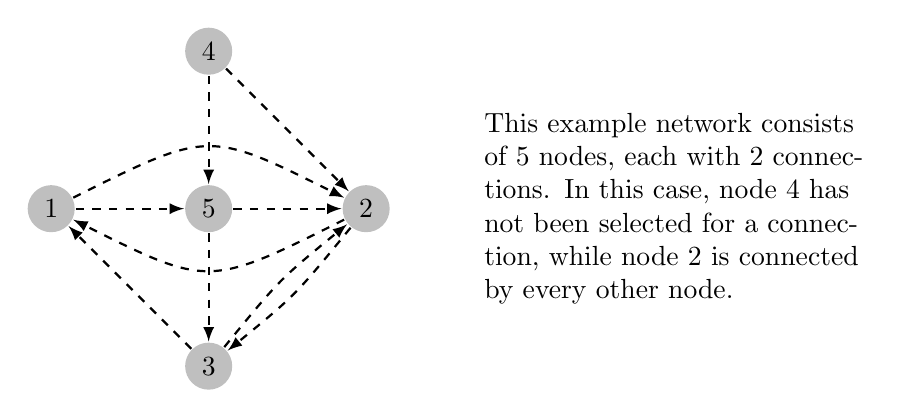
\begin{tikzpicture}[auto, thick]
				\tikzstyle{vertex}=[circle,fill=black!25,minimum size=17pt,inner sep=0pt]
				\node[vertex] (Node-1) at (-2,0) {$1$};
				\node[vertex] (Node-2) at (2,0) {$2$};
				\node[vertex] (Node-3) at (0,-2) {$3$};
				\node[vertex] (Node-4) at (0,2) {$4$};
				\node[vertex] (Node-5) at (0,0) {$5$};
				
				\draw[-latex, thick, dashed, black] (Node-1) .. controls (0,1) .. (Node-2);
				\draw[-latex, thick, dashed, black] (Node-1) -- (Node-5);
				
				\draw[-latex, thick, dashed, black] (Node-2) .. controls (0,-1) .. (Node-1);
				\draw[-latex, thick, dashed, black] (Node-2) .. controls (1.1,-1.1) .. (Node-3);
				
				\draw[-latex, thick, dashed, black] (Node-3) .. controls (0.9,-0.9) .. (Node-2);
				\draw[-latex, thick, dashed, black] (Node-3) -- (Node-1);
				
				\draw[-latex, thick, dashed, black] (Node-4) -- (Node-2);
				\draw[-latex, thick, dashed, black] (Node-4) -- (Node-5);
				
				\draw[-latex, thick, dashed, black] (Node-5) -- (Node-3);
				\draw[-latex, thick, dashed, black] (Node-5) -- (Node-2);
				
				\node[text width=5cm] at (6,0) {This example network consists of 5 nodes, each with 2 connections. In this case, node 4 has not been selected for a connection, while node 2 is connected by every other node.};
				
				%\draw[-latex, thick, dashed, black] (Node-2) -- (Node-1);
				\end{tikzpicture}	
				
				\caption{High-level internodal connection diagram example}
				\label{fig:internodalexample}
				%\end{center}
			\end{figure}
			
			
			
			
			
			
			
			
			
			
			
			
			
			
			
			
			
			
			
		\subsubsection{Packet Classes}
			\begin{description}[topsep=-5pt,itemsep=-1ex,partopsep=2ex,parsep=1.5ex]
				\item[Data as Notifications] \hfill \\
				A single class of data packet is used, where the intended message and notification of the existence of said message are combined. This means that if a notification is successful, the data will always be available, resulting in lower delivery latency. However, as the size of some packets could be large, and the majority of this information is destined for most nodes, this is likely to be wasteful and could cause scalability issues.
				\item[Notifications Referencing Data] \hfill \\
				Two classes of packet are used: a data packet that is just for storing data and a notification packet that is only for notifying a node about the existence of a data packet. While all nodes still need to check all the notifications, only a subset of all nodes need to be in possession of the data packets. In addition, the notifications may also include information such as some known locations of the desired data packet (rendezvous nodes). This method has the potential to reduce the availability of data packets that are not distributed well throughout the network.
				\item[Notifications with Small Payload] \hfill \\
				Each notification packet is a union\footnote{A union type is one that provides an either-or contents structure.} of a small payload or a data packet reference. The total size of this is still comparable to that of a typical notification packet. The result of this structure would be very high availability for any small payload.
			\end{description}
			Given that notifications with small payloads have the potential to provide maximal flexibility while also reducing the load on the network, these will be used.
			
		\subsubsection{Information Distribution and Delivery}
			Distributing the information across the network must occur in order to keep the availability of information high. In order to receive a message, everyone must either check every message, or there must be some form of delegation to a third party, or parties, that must perform the same role.
			
			Systems, such as Bitmessage, take the approach that everyone can attempt to determine if a message is for them, whereas other systems, such as email, take advantage that the recipient of a message can be determined and use this to place the message in a predictable location. Other networks, such as Freenet, move the obligation of notification to out-of-band communications, meaning they do not address this issue.
			
			As the Bitmessage network grows, it splits into ``streams''~\cite{bitmsg}, effectively creating smaller subnetworks. Membership of a stream can be a function of some identifying element of the user, such as a public key (figure \ref{fig:stream-normal}). Although this method is promising in terms of scalability, it has some disadvantages for the anonymity of the network. This type of optimisation is only possible where each stream has enough members such that if the stream was isolated, the property of anonymity would hold. Under the assumption that one user controls exactly one node, it is enough for the node membership under any stream for be sufficiently high. However, if this assumption cannot be made, then it opens the possibility to deanonymisation attacks. The worst-case for this attack is that it may be possible to determine the public key, and therefore the identity that a node is interested in retrieving messages for. This would occur where an adversary is able to isolate a node in a stream (figure \ref{fig:stream-malicious}) and could happen where an adversary creates a large number of nodes with similar public keys (through trial and error, or otherwise) to the target node. Although this may only reveal the recipient's identity for new packets in the stream where the isolation attack is taking place, it is still undesirable.
			
			% Diagrams produced from modified code originally made by andrino Claudio 2011 - http://claudiofiandrino.altervista.org/

\definecolor{pinegreen}{cmyk}{0.92,0,0.59,0.25}
\definecolor{royalblue}{cmyk}{1,0.50,0,0}
\definecolor{lavander}{cmyk}{0,0.48,0,0}
\definecolor{violet}{cmyk}{0.79,0.88,0,0}

\tikzstyle{legend_overlay}=[rectangle, rounded corners, thin,
top color= white,bottom color=white, draw=black,
minimum width=2.5cm, minimum height=0.8cm,
black,rotate=90]
\tikzstyle{legend_general}=[rectangle, rounded corners, thin,
top color=white,bottom color=white, draw=black,
minimum width=2.5cm, minimum height=0.8cm,
black]
\begin{figure}
	\centering
	\begin{tikzpicture}[auto, thick]
	\tikzstyle{vertex}=[circle,fill=black!25,minimum size=17pt,inner sep=0pt]

	\node[legend_overlay] at (-6.5,0){\textsc{Before Split}};
	\node[legend_overlay] at (-6.5,-5){\textsc{After Split}};
	
	\node[cloud, draw=black, cloud puffs=16, cloud puff arc= 100, minimum width=7cm, minimum height=4.5cm, aspect=1] (Stream-main) at (0,0) {};
	\node[legend_general] at (0,1.6){Stream for PKs 0* to f*};
	\foreach \name/\y/\pk in {a/0/PK: 0fa79\ldots, b/0.7/PK: c2955\ldots, c/1.4/PK: 3795a\ldots, d/2.1/PK: ee775\ldots} {
		\node[vertex] (A-\name) at (-1.3,0.8-\y) {$\name$};	\node[right] (A-label-a) at (-1,0.8-\y) {$\pk$};
	}
	
	\node[cloud, draw=black, cloud puffs=16, cloud puff arc= 100, minimum width=5cm, minimum height=3.5cm, aspect=1] (Stream-split1) at (-3,-5) {};
	\node[legend_general] at (-3,-3.9){{Stream for PKs 0* to 7*}};
	\foreach \name/\y/\pk in {a/0/PK: 0fa79\ldots, c/0.7/PK: 3795a\ldots} {
		\node[vertex] (B-\name) at (-4.3,-5-\y) {$\name$};	\node[right] (B-label-a) at (-4,-5-\y) {$\pk$};
	}
	
	\node[cloud, draw=black, cloud puffs=16, cloud puff arc= 100, minimum width=5cm, minimum height=3.5cm, aspect=1] (Stream-split2) at (3,-5) {};
	\node[legend_general] at (3,-3.9){{Stream for PKs 8* to f*}};
	\foreach \name/\y/\pk in {b/0/PK: c2955\ldots, d/0.7/PK: ee775\ldots} {
		\node[vertex] (C-\name) at (1.7,-5-\y) {$\name$};	\node[right] (C-label-a) at (2.0,-5-\y) {$\pk$};
	}
	
	\draw[-latex, thick, black] (Stream-main) -- (Stream-split1);
	\draw[-latex, thick, black] (Stream-main) -- (Stream-split2);
	\end{tikzpicture}
	\caption{Example of intended stream usage}
	\label{fig:stream-normal}
%	\end{center}
\end{figure}


\begin{figure}
	\centering
	\begin{tikzpicture}[auto, thick]
	\tikzstyle{vertex}=[circle,fill=black!25,minimum size=17pt,inner sep=0pt]
	
	\node[cloud, fill=white, draw=black, cloud puffs=16, cloud puff arc= 100, minimum width=7cm, minimum height=4.5cm, aspect=1] at (0,0) {};
	\node[legend_general] at (0,1.6){{Stream for PKs 0fa*}};
	
	\foreach \name/\y/\pk in {E/0/PK: 0fa73\ldots, F/0.7/PK: 0fa18\ldots, H/2.1/PK: 0fa9c\ldots} {
		\node[vertex, fill=black!70!white, text=white] (A-\name) at (-1.3,0.8-\y) {$\name$};
		\node[right, text=black] (A-label-a) at (-1,0.77-\y) {$\pk$};
	}
	
	\foreach \name/\y/\pk in {g/1.4/PK: 0faf2\ldots} {
		\node[vertex] (A-\name) at (-1.3,0.8-\y) {$\name$};
		\node[right] (A-label-a) at (-1,0.8-\y) {$\pk$};
	}
	\end{tikzpicture}
	\caption{Example of malicious nodes isolating a legitimate node}
	\label{fig:stream-malicious}
	%\end{center}
\end{figure}


%\begin{figure}
%	\centering
%	\begin{tikzpicture}[auto, thick]
%	\tikzstyle{vertex}=[circle,fill=black!25,minimum size=17pt,inner sep=0pt]
%		\node[vertex] (Node-1) at (-2,0) {$1$};
%		\node[vertex] (Node-2) at (2,1.5) {$2$};
%		\node[vertex] (Node-3) at (2,0) {$3$};
%		\node[vertex] (Node-4) at (2,-1.5) {$4$};
%		
%		\node[vertex] (Node-X) at (5,2) {$X$};
%		\node[right] (Node-label-X) at (5.5,2) {Node X};
%		
%	\tikzstyle{vertex}=[circle,fill=yellow!25,draw=black,minimum size=12pt,inner sep=0pt]
%		
%		\node[vertex] (Packet-y) at (5,1.2) {$y$};
%		\node[right] (Packet-label-y) at (5.5,1.2) {Packet y};
%	
%		\node[vertex] (Packet-1-a) at (-2.5,0.5) {$a$};
%		\node[vertex] (Packet-1-b) at (-2.7,0) {$b$};
%		%\node[vertex] (Packet-1-c) at (-2.5,-0.5) {$c$};
%		\draw[thick, black] (Node-1) -- (Packet-1-a);
%		\draw[thick, black] (Node-1) -- (Packet-1-b);
%		%\draw[thick, black] (Node-1) -- (Packet-1-c);
%		
%		\node[vertex] (Packet-2-a) at (2.5,2) {$a$};
%		\node[vertex] (Packet-2-b) at (2.7,1.5) {$b$};
%		\draw[thick, black] (Node-2) -- (Packet-2-a);
%		\draw[thick, black] (Node-2) -- (Packet-2-b);
%		
%		\node[vertex] (Packet-3-a) at (2.5,0.5) {$a$};
%		\node[vertex] (Packet-3-c) at (2.7,0) {$c$};
%		\draw[thick, black] (Node-3) -- (Packet-3-a);
%		\draw[thick, black] (Node-3) -- (Packet-3-c);
%		
%		\node[vertex] (Packet-4-b) at (2.5,-1) {$b$};
%		\node[vertex] (Packet-4-d) at (2.7,-1.5) {$d$};
%		\draw[thick, black] (Node-4) -- (Packet-4-b);
%		\draw[thick, black] (Node-4) -- (Packet-4-d);
%		
%		\node[text width=5cm] at (6,-1) {Node 1 selects nodes 2 and 3 to be its connections into the network};
%		
%		\draw[-latex, thick, dashed, black] (4.5,0.4) -- (5.4,0.4);
%		\node[right] (Arrow) at (5.5,0.4) {Connection};
%		
%		\draw[-latex, thick, dashed, black] (Node-1) -- (Node-2);
%		\draw[-latex, thick, dashed, black] (Node-1) -- (Node-3);
%		%\node[right] (A-label-a) at (-1,0.8-\y) {$\pk$};
%	\end{tikzpicture}	
%	
%	\vspace*{0.1cm} \hrulefill \vspace*{0.1cm}
%	
%		\begin{tikzpicture}[auto, thick]
%		\tikzstyle{vertex}=[circle,fill=black!25,minimum size=17pt,inner sep=0pt]
%		\node[vertex] (Node-1) at (-2,0) {$1$};
%		\node[vertex] (Node-2) at (2,1.5) {$2$};
%		\node[vertex] (Node-3) at (2,0) {$3$};
%		\node[vertex] (Node-4) at (2,-1.5) {$4$};
%		
%		\tikzstyle{vertex}=[circle,fill=yellow!25,draw=black,minimum size=12pt,inner sep=0pt]
%		
%		\node[vertex] (Packet-1-a) at (-2.5,0.5) {$a$};
%		\node[vertex] (Packet-1-b) at (-2.7,0) {$b$};
%		\node[vertex] (Packet-1-N) at (-2.5,-0.5) {$N$};
%		\draw[thick, black] (Node-1) -- (Packet-1-a);
%		\draw[thick, black] (Node-1) -- (Packet-1-b);
%		\draw[thick, black] (Node-1) -- (Packet-1-N);
%		
%		\node[vertex] (Packet-2-a) at (2.5,2) {$a$};
%		\node[vertex] (Packet-2-b) at (2.7,1.5) {$b$};
%		\draw[thick, black] (Node-2) -- (Packet-2-a);
%		\draw[thick, black] (Node-2) -- (Packet-2-b);
%		
%		\node[vertex] (Packet-3-a) at (2.5,0.5) {$a$};
%		\node[vertex] (Packet-3-c) at (2.7,0) {$c$};
%		\draw[thick, black] (Node-3) -- (Packet-3-a);
%		\draw[thick, black] (Node-3) -- (Packet-3-c);
%		
%		\node[vertex] (Packet-4-b) at (2.5,-1) {$b$};
%		\node[vertex] (Packet-4-d) at (2.7,-1.5) {$d$};
%		\draw[thick, black] (Node-4) -- (Packet-4-b);
%		\draw[thick, black] (Node-4) -- (Packet-4-d);
%		
%		\node[text width=5cm] at (6,0) {Node 1 inserts a new packet N into the network by forwarding it along the connections, using Nodes 2 and 3 as rendezvous points};
%		
%		\draw[thick, red] (Node-1) -- (Node-2);
%		\draw[thick, red] (Node-1) -- (Node-3);
%		
%		\draw[-latex, thick, dashed, black] (Node-1) -- (Node-2);
%		\draw[-latex, thick, dashed, black] (Node-1) -- (Node-3);
%		%\node[right] (A-label-a) at (-1,0.8-\y) {$\pk$};
%		\end{tikzpicture}
%	
%	
%	
%	\caption{TEST}
%	\label{fig:TEST}
%	%\end{center}
%\end{figure}















			
			While all nodes need to check all messages to a degree, this mechanism is only required to notify of a message. Hence, instead of combining the notification and data functionality in a single packet, and having everyone acquire all of these, a split can be made. This would still require everyone to acquire and check all the notification packets, but these notifications could point to a data packet elsewhere on the network, along with a collection of rendezvous nodes that are known to be in possession of these data packets.
			
			\subsubsection{Broadcast Handling}
			Notifications will be broadcast to at least all nodes that are members of a stream, this is likely to be the bottleneck of the system. The handling of broadcasts should therefore be subject to optimisation where possible.

			\begin{description}[topsep=-5pt,itemsep=-1ex,partopsep=2ex,parsep=1.5ex]
				\item[Universal Polling (UP)] \hfill \\
				Nodes query other nodes for a list of their stored broadcasts, acting like a distributed hash table. The querying node can then request any broadcast it does not have stored. If the rate of broadcasts inserted into the network is greater than the rate they expire, then the size of the query response will grow unsustainably.
				\item[Active Forwarding (AF)] \hfill \\
				Upon receiving a broadcast for the first time, the node forwards it to all of its connections. This does not require any list of broadcasts to be distributed, saving on some overhead. However, as the node initiating the forwarding is unaware if the nodes are in possession of the broadcast, the receiving node will be responsible for signalling that further transfer is not required, probably in the form of terminating the connection.
				\item[Selective Polling (SP)] \hfill \\
				When a node receives a broadcast, it also stores the time of receipt. When a node polls another node, it stores the time of polling for that node. In a similar way to UP, polling is used to gather a list of broadcasts, but a parameter specifying the last time of polling is passed too. The polled node returns the list of all broadcasts that it received after this time. This has potential anonymity implications where it may reveal the time at which a node received a broadcast. However, this can be negated by having the receiving node add a small random time to the real time of receipt.
			\end{description}
			\begin{figure}
	\centering
		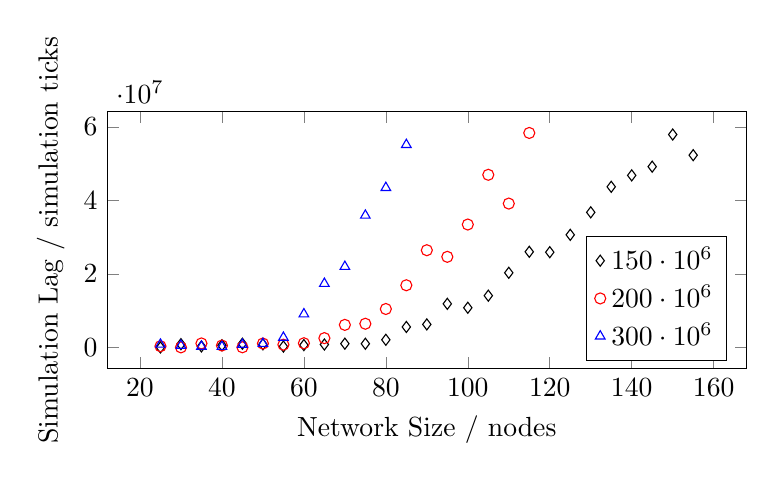
\begin{tikzpicture}
			\begin{axis}[
					width=0.8\linewidth,
					height=0.4\linewidth,
					xlabel=Network Size / nodes,
					ylabel=Simulation Lag / simulation ticks,
					legend entries={$150\cdot10^6$, $200\cdot10^6$, $300\cdot10^6$},
					legend pos=south east
				]
			%	\addlegendentry{\hspace{-.6cm}\textbf{Time}}
				\addplot[
					scatter,
					only marks,
					point meta=explicit symbolic,
					scatter/classes={
						a={mark=diamond,black},
						b={mark=o,draw=red},
						d={mark=triangle,blue}
						},
				]
				table[meta=label] {
					x y label
					25	24541 a
					30	907572 a
					35	304920 a
					40	616387 a
					45	1031117 a
					50	864221 a
					55	258485 a
					60	653754 a
					65	809943 a
					70	1048788 a
					75	1026927 a
					80	2100095 a
					90	6288081 a
					85	5590600 a
					95	11880910 a
					100	10815227 a
					105	14100952 a
					110	20324960 a
					115	26029089 a
					125	30645860 a
					120	25923148 a
					130	36772925 a
					135	43713637 a
					140	46817286 a
					150	57932035 a
					145	49191305 a
					155	52311392 a
					25	357262 b
					30	33972 b
					35	1112397 b
					40	540416 b
					45	61033 b
					50	1082894 b
					55	775513 b
					60	1163609 b
					65	2553731 b
					70	6156550 b
					75	6463167 b
					80	10478434 b
					85	16933039 b
					95	24665926 b
					90	26465847 b
					110	39154681 b
					100	33453911 b
					115	58362416 b
					105	46980354 b
					25	846698 d
					35	269968 d
					30	541413 d
					40	228635 d
					45	811461 d
					50	1057005 d
					55	2725045 d
					60	9102614 d
					65	17391255 d
					70	22003664 d
					80	43466949 d
					75	35927541 d
					85	55167398 d	
				};
			\end{axis}
		
		\end{tikzpicture}
		\caption{Simulation lag for network sizes for varying simulation lengths (UP)}
		\label{fig:simulation-lag}
	%\end{center}
%\end{figure}
	\vspace*{1cm}
%\begin{figure}
	\centering
		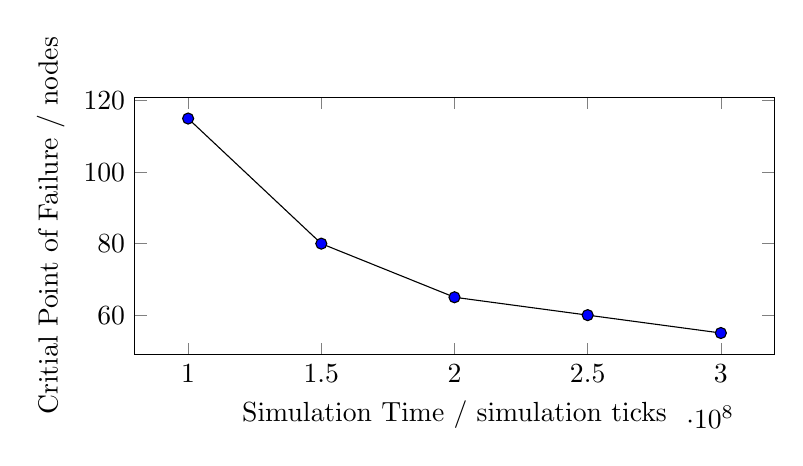
\begin{tikzpicture}
		\begin{axis}[
			width=0.8\linewidth,
			height=0.4\linewidth,
			xlabel=Simulation Time / simulation ticks,
			ylabel=Critial Point of Failure / nodes,
			xtick={100e6,150e6,200e6,250e6,300e6}
		]
		\addplot[
		scatter,
		scatter/use mapped color={draw=none, fill=blue}
		]
		table {
			x y
			100e6	115
			150e6	80
			200e6	65
			250e6	60
			300e6	55
		};
		\end{axis}
		\end{tikzpicture}
		\caption{Critical point of failure for simulation lengths (UP)}
		\label{fig:critical-point}
	%\end{center}
%\end{figure}
	\vspace*{1cm}
%\begin{figure}
	\centering
		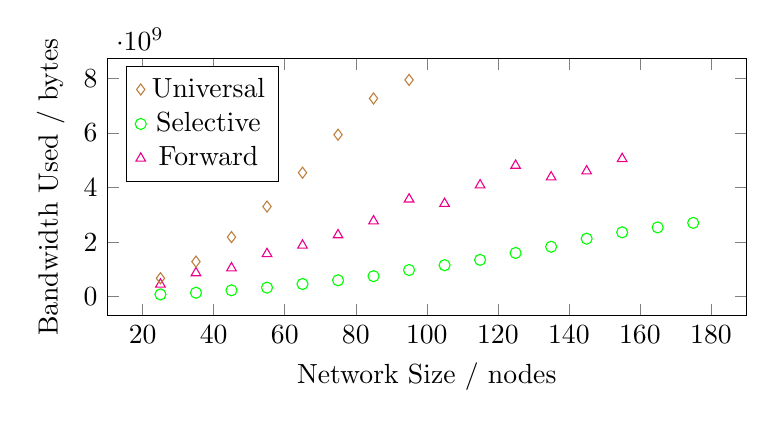
\begin{tikzpicture}
		\begin{axis}[
		width=0.8\linewidth,
		height=0.4\linewidth,
		xlabel=Network Size / nodes,
		ylabel=Bandwidth Used / bytes,
		legend entries={Universal, Selective, Forward},
		legend pos=north west
		]
		%	\addlegendentry{\hspace{-.6cm}\textbf{Time}}
		\addplot[
		scatter,
		only marks,
		point meta=explicit symbolic,
		scatter/classes={
			universal={mark=diamond,brown},
			selective={mark=o,draw=green},
			forward={mark=triangle,magenta}
		},
		]
		table[meta=label] {
			x y label
			25 456019780 forward
			35 872253165 forward
			45 1048887570 forward
			55 1573692515 forward
			65 1881124400 forward
			75 2262434505 forward
			85 2771544750 forward
			95 3573927345 forward
			105 3411036380 forward
			115 4092502880 forward
			125 4807955340 forward
			135 4384191915 forward
			145 4602090000 forward
			155 5055210185 forward

			25 677312540 universal
			35 1287235525 universal
			45 2185638925 universal
			55 3304297955 universal
			65 4545322280 universal
			75 5936811385 universal
			85 7265776430 universal
			95 7945404335 universal
			
			25 85397100 selective
			35 147088405 selective
			45 235060850 selective
			55 333573715 selective
			65 466682360 selective
			75 602788785 selective
			85 754004910 selective
			95 979054255 selective
			105 1156023540 selective
			115 1351527220 selective
			125 1604653050 selective
			135 1832297135 selective
			145 2127906425 selective
			155 2361108570 selective
			165 2540262770 selective
			175 2706737490 selective
		};
		\end{axis}
		
		\end{tikzpicture}
		\caption{Bandwidth used for different broadcast handling methods near steady-state}
		\label{fig:bandwidth-required}
\end{figure}
			Simulations for each of the 3 broadcast handling methods were run for a set period of time. For the interval up to this time, nodes are stimulated, adding tasks for them to perform, such as querying another node or pushing data into the network. After the allowed simulation time, no more stimulations occur and the remaining tasks are allowed to complete. The interval from stopping stimulations to the end of the simulation is referred to as the simulation lag. More detail on the simulator can be found in appendix \ref{simulator}. It should be noted that time, in this context, is measured in simulation ticks, not the real time the simulation takes to complete. Small simulation lag values are what is expected to result from a sustainable system where tasks do not accumulate.
			
			Simulation results are not absolute, and real scalability and performance results will be dependant on real network usage. The simulations presented here, subject to minor variation in the random nature of simulating usage, have been conducted under the same usage conditions.
			
			Running the simulation for UP for a set time, while varying the size of the network results in the graph shown in figure \ref{fig:simulation-lag}. The point where the method fails for a simulation interval of $150\cdot10^6$ ticks, can be seen to occur at 80 nodes. For UP, the points of failure for different simulation times were plotted, as shown in figure \ref{fig:critical-point}. This downward trend indicates that the number of nodes needed for network failure decreases the longer the network is active.
			
			Simulations for SP and AF were also conducted, but points of failure could not be determined.
			
			The simulations were run for $300\cdot10^6$ ticks, to achieve near steady-state behaviour in the network. The bandwidth used over each of the simulations was compared, as shown in figure \ref{fig:bandwidth-required}. A possible reason for AF having worse performance than SP is that when multiple nodes forward the same packet to the same node, a race condition is effectively created (figure \ref{fig:activefail}).
			
			While optimisations for AF can prevent this race condition by informing any receiving nodes of the forwarded packet ID before the packet contents and allowing only one incoming connection for each unique packet, this has the potential to open up an attack vector for a denial of service where a malicious node could easily forward a genuine packet at a very slow speed, therefore significantly increasing latency for a given node.
			
			\begin{figure}
				\centering
				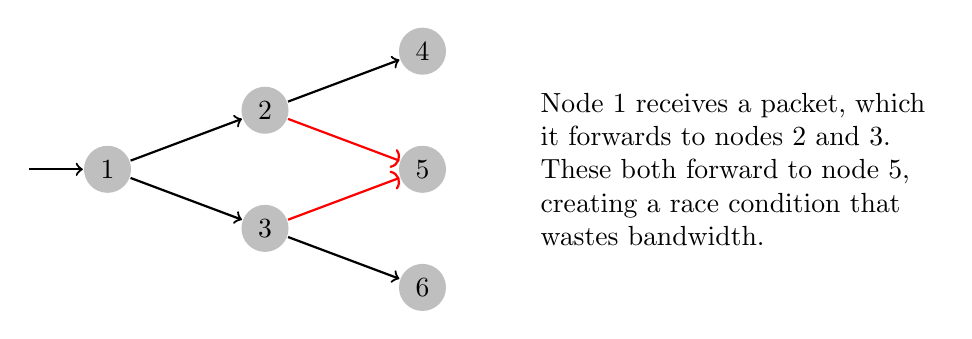
\begin{tikzpicture}[auto, thick]
				\tikzstyle{vertex}=[circle,fill=black!25,minimum size=17pt,inner sep=0pt]
				\node[vertex] (Node-1) at (-2,0) {1};
				\node[vertex] (Node-2) at (0,0.75) {2};
				\node[vertex] (Node-3) at (0,-0.75) {3};
				\node[vertex] (Node-4) at (2,1.5) {4};
				\node[vertex] (Node-5) at (2,0) {5};
				\node[vertex] (Node-6) at (2,-1.5) {6};
				
				\draw[->, thick, solid, black] (-3,0) -- (Node-1);
				
				\draw[->, thick, solid, black] (Node-1) -- (Node-2);
				\draw[->, thick, solid, black] (Node-1) -- (Node-3);
				
				\draw[->, thick, solid, black] (Node-2) -- (Node-4);
				\draw[-), thick, solid, red] (Node-2) -- (Node-5);
				
				\draw[->, thick, solid, black] (Node-3) -- (Node-6);
				\draw[-), thick, solid, red] (Node-3) -- (Node-5);
				
				\node[text width=5cm] at (6,0) {Node 1 receives a packet, which it forwards to nodes 2 and 3. These both forward to node 5, creating a race condition that wastes bandwidth.};
				
				%\draw[-latex, thick, dashed, black] (Node-2) -- (Node-1);
				\end{tikzpicture}	
				
				\caption{Active forwarding wasted bandwidth caused by race condition}
				\label{fig:activefail}
				%\end{center}
			\end{figure}
			
			SP has the potential to require the least bandwidth for broadcasts. AF may also be useful to support for the purpose of initial packet distribution, to both increase availability faster and to increase anonymity by hiding the original source of packets.
			
		
	\subsection{API} % STATUS: Complete & Checked
		% STATUS: Complete & Checked
		The primary objective of the system is to provide an API for a send-receive architecture, affording the sending and receipt of messages. The node implementation and abstract protocol are therefore designed around this objective.
		
		% STATUS: Complete & Checked
		The API is designed to revolve around two functions: send and receive. Sending requires knowledge of the public identity of the receiver; the message and how long it should be stored in the network. Receiving requires knowledge of a private identity, which returns a message for the given identity. Both functions are blocking, meaning that sending will block until the message is in the network and receiving will block until a message that has not been received previously is returned. Appendix \ref{uml-api} shows the general design for the API.
	\subsection{Abstract Protocol} % STATUS: Complete
		The UML for the protocol can be found in appendix \ref{uml-protocol}.

The network is made up of both participating nodes, and non-participating nodes. Participating nodes need to provide some method of creating and handing requests (figure \ref{fig:protointernodalconusecase}) for: 
\begin{itemize}[topsep=-5pt,itemsep=-1ex,partopsep=2ex,parsep=1.5ex]
	\item The active nodes they know about
	\item The packets they are in possession of, and the class of these packets
	\item The acceptable proof-of-work and cryptographic algorithms that are accepted
	\item The acquisition of a packet given the packet's ID
\end{itemize} \vspace{0.7ex}

% STATUS: Complete & Checked
% DOUBTS: Slightly disjoint
Each participating node in the network has a psuedoidentifier, which is assumed to be unique, and allows connections to be made to the node, using it as an address. To facilitate the discovery of nodes in the network, nodes are initially provided with at least one psuedoidentifier of a node in the network, allowing an initial point of contact. The acquisition of the initial nodes' psuedoidentifiers occurs out-of-band.

% STATUS: Complete & Checked
% DOUBTS: Maybe reword?
Each node is classified into one of 4 categories: active, where the node is online and responding the requests normally; inactive, where the node appears to be offline; unknown, where the node is yet to be tested for activity; undiscovered, where the node has not been discovered or referenced. All newly discovered nodes are considered unknown and tested to reclassify them as either active or inactive. Active nodes can then be used for connections, creating multiple unidirectional links to the network. Should an active node appear to be inactive by not responding appropriately, it shall be reclassified as inactive. Inactive nodes are periodically checked for signs of activity and reclassified if necessary. %\todo[inline]{Flow for classification?}

%Information about packet possession is achieved through selective polling. Each node holds some mapping from nodes to timestamps, which relates to the last time that the mapped node was polled. This timestamp is sent with any polling request, therefore ensuring the list of packets the polled node lists is composed purely of new information. \todo[inline]{Polling seq diagram}

%\todo{Move to elements?}While to process of inserting a packet into the network could easily be achieved through just possessing the packet and letting other nodes retrieve it, this both increases the period of distribution (decreasing immediate availability), and as the packet will originate from a single node, may allow the origin of a packet to be determined.

% STATUS: Complete & Checked
Three packet classes are used in the protocol: meta packets, for the exchange of internal information between nodes; data packets, for the representation of large messages; and broadcast packets, to represent small messages, or to act as a notification of the existence of a data packet.

% STATUS: Complete & Checked
% DOUBTS: Secondary footnote
In order to achieve predictable availability in the network, the lifetime of packets is controlled through the use of time-sensitive proof-of-works. A packet is only considered valid if also accompanied by a valid proof-of-work and packets should only be processed or stored if they are valid. Distribution for broadcast packets is universal, but the maximum broadcast size is small\footnote{\label{fn:imp-detail}Implementation detail.} and implementations may required a more difficult proof-of-work for broadcasts. Data packets, with a larger maximum size, are not universally distributed, but rather, distributed to some subset of nodes in the network, referred to as rendezvous nodes. These rendezvous nodes can then be listed in a notification packet.

% STATUS: Complete & Checked
Packet distribution in the network is accomplished mainly with selective polling to determining packet ownership, with requests to download new packets. Packet forwarding is also permitted, and any valid packet that is forwarded should be stored. While not a requirement of the protocol, it is allowable to use selective polling with download requests to acquire arbitrary data packets. As the main distribution mechanism for data packets is forwarding from the source node, this creates somewhat of a network-hard proof-of-work requirement for the sender, where the availability (as a function of the nodes that own the packet) increases with bandwidth used.

% STATUS: Complete & Checked
% DOUBTS: Could mention store-retrieve, but maybe not...
If utilising the send-receive architecture of the network, the insertion of a valid data packet into the network will also require the insertion of at least one valid broadcast packet, whose purpose will be to inform the recipient of the ID of the data packet, any associated encryption key and the identity of the  rendezvous nodes on which the data packet is known to exist. Multiple recipients can be achieved by inserting a broadcast packet for each recipient.

% STATUS: Complete
Packet receipt is attained through the acquisition and inspection of all valid broadcast packets. Any broadcast determined to be for the node is used for the message within the packet, or to determine the location of a referenced data packet. Referenced data packets can be acquired by downloading the packet at a rendezvous node specified in the broadcast, or a node that has been observed with selective polling to own the packet.

% STATUS: Complete
Streams allow the network to split into smaller subnetworks, with a split occurring once the condition that all streams after a potential split could still be considered anonymous, that is, if their membership still remains high. Membership of a stream is a function of some public value associated with the node. Each stream acts independently for the purpose of broadcast distribution, with cross-stream communications permitted for the insertion of a packet into the stream where the recipient is known to reside.	
			
\section{Implementation and Testing}
	\subsection{Implementation}
		The implementation for the protocol has been named Stor, providing a backend to handle the protocol communications and an API which can be used by other applications wishing to use the network for anonymous communications.
		\subsubsection*{Licensing}
			As one of the core aims of the project is to release the code for Stor and its API, software licensing must be taken into account to not only ensure that anyone wishing to use the code can do so, but also to ensure that any third party code used is licensed to allow its use within this project.
		\subsubsection*{External Libraries}
			\begin{description}
				\item[net.freehaven.tor.control] BSD Licnese \\
					Provides a high-level interface for communicating with Tor's control port.
				\item[org.eclipse.jetty] Apache 2.0 and Eclipse Public License \\
					An embedded webserver that allows delegation of request handling.
				\item[org.apache.commons] Apache 2.0 License \\
					Provides various collections and utility classes.
				\item[com.google.code.mimeparse] MIT License \\
					A utility for parsing mime types for HTTP request acceptance.
				\item[tinfoil \textit{TorLib}] MIT License \\
					Provides a method for performing .onion address resolution.
				\item[com.google.gson] Apache 2.0 License \\
					Provides serialisation/deserialisation for JSON.
				\item[org.hsqldb] BSD License
					An embedded SQL database that provides encrypted data persistence.
				\item[com.google.protobuf] BSD License \\
					A high-efficency data structure serialiser.
			\end{description}
		\subsubsection*{Tor Interface}
			The interface to Tor was the first element to be implemented \todo{Move to mngmt?} due to the importance of its role in the project.
			
			This module communicates with a Tor instance in order to create hidden services programmatically. Bundling a Tor instance with Stor nodes was considered, but given the complications regarding keeping the instance up to date with the latest Tor releases when included in a package and potential conflicts arising from running multiple instances on a single system, it was decided that responsibility of running an instance should be deligated beyond the API for now.
			
			Tor provides an option to enable a control port, allowing the post-startup configuration. This control port is only bound locally and can use authentication to ensure any connections are legitimate. This interface module uses the Tor controller from \todo{Add Name} to connect the control port of a Tor instance. The module allows for password authentication with the control port using the password in the \textit{stor.cfg} configutation file. \todo[inline]{Could add information about how passwords are created? Maybe the password structure too.}
		\subsubsection*{RESTful API}
			Network implimentation is designed to provide a RESTful interface between nodes through the use of HTTP and JSON. With the use of these common technologies
		\subsubsection*{Persistence Layer}
			HSQLDB has been used to provide a layer of persistence for Stor nodes. This database allows local storage without running of a daemon and hence requires no setup from the user.
			
			Ideally, any data held as part of the persistence would be stored encrypted to prevent an adversary with disk access from determining any prior usage. HSQLDB provides database encryption, which uses a user-supplied password on node startup, if desired. Unfortantely, the encryption method used is somewhat weak in that patterns can be determined in the database, such as fields that contain the same values. While not ideal, HSQLDB's built-in encryption has been used to provide some protection.
			
			\todo[inline]{Could include details about database setup/running}
	\subsection{Demonstration}
		To demonstrate the API in action, 2 applications have been created. Application A, the sender, knows the identity of application B, and once the API has started the node, prompts for an input, which is fed into the API and inserted into the network for B to discover and retrieve.
		\todo[inline]{Demo}
	\subsection{Testing}
		The test plan for the teachinesting of the API can be found in appendix \ref{testplan}.
		\subsubsection*{Leakage of .onion Addresses}
			During testing, it was discovered that metadata was leaking through the form of hidden service DNS requests. This kind of problem is described in \cite{Thomas:2014:MLO:2665943.2665951}, where it is shown to be quite a widespread issue. For Stor, the leakage occurred because when using \textit{URLConnection}s, Java does not use any specified SOCKS proxy for address resolution, hence having the potential to leak information about which nodes are being connected to under some conditions.
			
			To resolve this, hidden service address resolution is handled separately to the proxy. The responsibility for this is partially handled by \textit{tinfoil.TorLib}, allowing Stor to pass a hidden service address to tor's resolver, which returns a local IP address that can then be used to make connections to the hidden service in the future without having to specify the hidden service address. This method ensures that no leakage occurs.
\section{Review and Future Work}

	\subsection{Management}
		For the first half of the project, during research, weekly meetings were complimented with reports detailing progress, problems and future targets. In the second half of the project, mainly during the implementation, meetings were generally replaced with email communication expressing progress and targets.
		
		Prior to extensive design work, an enumeration of the project elements was drafted and each briefly assessed and ranked for criticality, identifying tasks deemed critical for project success. Where possible, tasks assigned a high criticality index were approached first to ensure any issues with these tasks could be addressed with ample time.
		
		Throughout the project, multiple regular backups, including versioning have been made to off-site locations, providing several layers of redundancy. Work undertaken has been detailed in the log book in addition to weekly reports.

		Appendix \ref{sec:management} shows the Gantt charts detailing the predicted and realised time plans in addition to the risk assessment undertaken at the beginning of the project.
	\subsection{Critical Evaluation}
		The project has been quite successful in achieving the original goals: a framework for sending and receiving messages anonymously and asynchronously has been designed, implemented and released under a FOSS license. 
		
		As with any product making claims about security, it is necessary for independent audit to investigate the source code. 
		
		Several features that have been investigated in the design were not implemented. Streams were originally intended to be supported, but due to the security considerations of having a small network initially, where there is high potential for isolation attacks, this will be left for an extension as the network grows. Zeroisation of keys was identified and investigated for the node/API implementation, but not achieved due to technical limitations both with Java and some libraries included. While some zeroisation in some circumstances may occur, no guarantee is made.
		
		Future work could address some of these unimplemented features and also further investigate some issues with trust in the network. Currently, the network is trustless, meaning that a node not following the protocol, such as not storing forwarded packets, is trusted as much as any other node, which is not ideal.
		
		Management of the project has been highly successful, through the use of short-term targets while taking into account longer-term goals, there has been no point where the project has fallen critically behind schedule.

		In the future, some work could be done to utilise the Stor API to create an application that would benefit from anonymous asynchronous communications.
		
		Ultimately, while Stor in its current form requires some attention to fine-tune the behaviour, potential for usability in applications remains high.

\newpage
\raggedright
\bibliographystyle{plain}
\bibliography{report}

\appendix

\vspace*{\fill}
\begin{figure}[!hbt]
	\begin{center}
		\begin{tikzpicture} % [show background grid ]
		
		\umlclass[simple=false,type=class,x=0,y=1]{StorAPI}{stor : StorNode}{send(identity : PublicIdentity, message : binary)\\receive(identity : PrivateIdentity) : binary}
		\umlclass[simple=false,type=abstract,x=0,y=-7]{Identity}{}{}
		\umlclass[simple=false,type=abstract,x=4,y=-4]{PublicIdentity}{}{\umlvirt{encrypt(data : binary) : binary}}
		\umlclass[simple=false,type=abstract,x=-4,y=-4]{PrivateIdentity}{}{\umlvirt{decrypt(data : binary) : binary}}
		
		\umluniaggreg[attr1=1|sends for, attr2=0..*|,pos1=0.2,pos2=1.0]{StorAPI}{PublicIdentity}
		
		\umluniaggreg[attr1=1|listens for, attr2=0..*|,pos1=0.2,pos2=0.8]{StorAPI}{PrivateIdentity}
		
		\umlcompo[attr1=1|, attr2=1|]{Identity}{PublicIdentity}
		
		\umlcompo[attr1=1|, attr2=1|]{Identity}{PrivateIdentity}
		\end{tikzpicture}
	\end{center}
	\caption{API Class Diagram\label{fig:api-uml-design}}
\end{figure}
\vspace*{\fill}
\begin{figure}[!hbt]
	\begin{center}
		\begin{tikzpicture}
		\begin{umlseqdiag}
		\umlobject[class=Application]{app}
		\umlobject[class=StorAPI,x=5]{api}
		\umlobject[class=StorNode,x=10]{node}
		
		\begin{umlcall}[op={send(msg,pubID)}, dt=5]{app}{api}
		\begin{umlcall}[op={applyFunction}]{api}{api}
		\end{umlcall}
		
		\begin{umlcall}[op={insert(appliedMsg)}]{api}{node}
		\end{umlcall}
		\end{umlcall}
		
		\end{umlseqdiag}
		\end{tikzpicture}
	\end{center}
	\caption{API Send Sequence Diagram}
\end{figure}
\vspace*{\fill}
\begin{figure}[!hbt]
	\begin{center}
		\begin{tikzpicture}
		\begin{umlseqdiag}
		\umlobject[class=Application]{app}
		\umlobject[class=StorAPI,x=5]{api}
		\umlobject[class=StorNode,x=10]{node}
		\begin{umlcall}[op={receive(priID)}, dt=5]{app}{api}
		\begin{umlfragment}[type=loop]
		\begin{umlcall}[op={check(appliedMsg)}, dt=10]{node}{api}
		\begin{umlcall}[op={inverse(appliedMsg)}]{api}{api}
		\end{umlcall}
		\end{umlcall}
		\end{umlfragment}
		\begin{umlfragment}[type=opt, label=for priID, inner xsep=8, fill=green!10]
		\begin{umlcall}[type=return, op=msg]{api}{app}
		\end{umlcall}
		\end{umlfragment}
		\end{umlcall}
		\end{umlseqdiag}
		\end{tikzpicture}
	\end{center}
	\caption{API Receive Sequence Diagram}
\end{figure}
\vspace*{\fill}
\begin{center}
		\begin{tikzpicture}
		\umlactor[y=1]{Node}
		\begin{umlsystem}[]{Internodal Communications}
		\umlusecase[x=10,y=0,fill=blue!10,name=reqinfo]{Request Info}
		\umlusecase[x=7,y=-1,fill=blue!10,name=reqpos]{Request Possession}
		\umlusecase[x=4,y=-2,fill=blue!10,name=reqnodes]{Request Nodes}
		
		\umlusecase[x=10,y=2,fill=green!10,name=resinfo]{Respond Info}
		\umlusecase[x=7,y=3,fill=green!10,name=respos]{Respond Possession}
		\umlusecase[x=4,y=4,fill=green!10,name=resnodes]{Respond Nodes}
		\end{umlsystem}
		
		\umlassoc{Node}{reqinfo}
		\umlassoc{Node}{reqpos}
		\umlassoc{Node}{reqnodes}
		\umlassoc{Node}{resinfo}
		\umlassoc{Node}{respos}
		\umlassoc{Node}{resnodes}
		
		\umlinclude[]{resinfo}{reqinfo}
		\umlinclude[]{resnodes}{reqnodes}
		\umlinclude[]{respos}{reqpos}
		
		\end{tikzpicture}
	\captionof{figure}{Protocol's Internodal Communications Use Case Diagram\label{fig:protointernodalconusecase}}
\end{center}
\begin{center}
		\begin{tikzpicture} % [show background grid ]
		
		\umlclass[simple=false,type=class,x=0,y=0]{Node}{pseudoidentity : Identifier}{}
		\umlclass[simple=true,type=abstract,x=7,y=0]{Packet}{}{}
		\umlclass[simple=true,type=class,x=7,y=-2]{MetaPacket}{}{}
		\umlclass[simple=false,type=class,x=5,y=3]{BroadcastPacket}{message : binary}{}
		\umlclass[simple=false,type=class,x=9,y=3]{DataPacket}{message : binary}{}
		
		\umlaggreg[attr1=0..*|, attr2=1|]{Packet}{Node}
		%\umlcompo[attr1=1|, attr2=1|]{Packet}{PacketPayload}
		
		\umlinherit{MetaPacket}{Packet}
		\umlinherit{BroadcastPacket}{Packet}
		\umlinherit{DataPacket}{Packet}
		
		\umlNarynode[x=5,y=6,name=ref,above]{Ownership Reference}
		\umlassoc[geometry=|-,attr1=|0..*]{Node}{ref}
		\umlassoc[geometry=|-,attr1=|0..1]{DataPacket}{ref}
		\umlassoc[attr1=has|1]{BroadcastPacket}{ref}
		
		\umlaggreg[angle1=-20, angle2=-50, loopsize=4cm, attr1=|1, attr2=knows about|1..*]{Node}{Node}
		
		\umlaggreg[angle1=-80, angle2=-130, loopsize=2cm, attr1=|1, attr2=connected to|1..*]{Node}{Node}
		
		\end{tikzpicture}
	\vspace*{-1.5cm}
	\captionof{figure}{Protocol Class Diagram}
\end{center}

\begin{center}
		\begin{tikzpicture}
		\begin{umlseqdiag}
		\umlobject[class=Node]{a}
		\umlobject[class=Node,x=6]{b}
		\begin{umlcall}[op={lookupTime(b)}]{a}{a}
			\begin{umlcall}[op={poll(time$_{a,b}$)},return={packet IDs}]{a}{b}
				\begin{umlcall}[op={lookupPacketsSince(time$_{a,b}$)}]{b}{b}
				\end{umlcall}
			\end{umlcall}
			
			\begin{umlcall}[op={storePacketIDs()}]{a}{a}
			\end{umlcall}
			\begin{umlcall}[op={updateTime(b)}]{a}{a}
			\end{umlcall}
		\end{umlcall}
		\begin{umlcall}[op={requestPacket(p)}, return={p}]{a}{b}
		\end{umlcall}
		\end{umlseqdiag}
		\end{tikzpicture}
	
	\captionof{figure}{Protocol Selective Polling Sequence Diagram\label{fig:pro-sp}}
\end{center}

\begin{center}
		\begin{tikzpicture}
		\begin{umlseqdiag}
		\umlobject[class=Node]{a}
		\umlobject[class=Node,x=6]{b}
		\begin{umlcall}[op={acquirePacket()}]{a}{a}
			\begin{umlcall}[op={forward(p)}]{a}{b}
			\end{umlcall}
		\end{umlcall}
		\end{umlseqdiag}
		\end{tikzpicture}
	
	\captionof{figure}{Protocol Active Forwarding Sequence Diagram\label{fig:pro:af}}
\end{center}
\begin{center}
		\begin{tikzpicture}
		\begin{umlseqdiag}
		\umlobject[class=Node]{x}
		\umlobject[class=Node,x=5]{y}
		
		\begin{umlcall}[op={requestNodes($addr_x$)}, return=active nodes to y]{x}{y}
		\begin{umlcall}[op={setUnknown($addr_x$)}]{y}{y}
		\end{umlcall}
		\end{umlcall}
		
		\begin{umlfragment}[name=check, type=alt, label={online}, inner xsep=5]
		\begin{umlcall}[op={requestInfo}, return=info, dt=8]{y}{x}
		\end{umlcall}
		\begin{umlcall}[op={setActive($addr_x$)}]{y}{y}
		\end{umlcall}
		\umlfpart[offline]
		\begin{umlcall}[op={requestInfo}]{y}{x}
		\end{umlcall}
		\begin{umlcall}[op={setInactive($addr_x$)}, dt=0]{y}{y}
		\end{umlcall}
		\end{umlfragment}
		%\umlnote[x=2, y=-11]{check}{Check node is active or not}
		\end{umlseqdiag}
		\end{tikzpicture}
	
	\captionof{figure}{Node Discovery Sequence Diagram\label{fig:node-discovery-seq}}
\end{center}

\begin{center}
	\begin{tikzpicture} % [show background grid ]
	
	\umlclass[simple=true,type=class,x=0,y=0]{Packet}{}{}
	\umlclass[simple=false,type=abstract,x=-3,y=-5]{ProofOfWork}{POWAlgorithm : algorithm\\PayloadHash : binary\\Proof : binary\\ValidFrom : timestamp\\ValidTo : timestamp}{}
	\umlclass[simple=false,type=abstract,x=3,y=-5]{Payload}{\umlvirt{classFlag : byte}\\message : binary}{}
	\umlclass[simple=true,type=class,x=-1,y=-9]{BroadcastPayload}{}{}
	\umlclass[simple=true,type=class,x=4,y=-9]{DataPayload}{}{}

	\umlcompo[attr1=1|, attr2=1|, pos2=0.5]{Packet}{ProofOfWork}
	\umlcompo[attr1=1|, attr2=1|, pos2=0.5]{Packet}{Payload}
	
	\umlinherit{BroadcastPayload}{Payload}
	\umlinherit{DataPayload}{Payload}
	\end{tikzpicture}
	\captionof{figure}{Node Packet Class Structure\label{fig:node-uml-class}}
\end{center}
%%Test Plan
\begin{landscape}
	\section{Test Plan} \label{testplan}
	
	\renewcommand{\arraystretch}{1.2}
	
	\subsection*{Unit Tests}
	\begin{table}[h]
		\begin{tabular}{| l | p{13cm} | l |}
			\hline
			Unit Test & Description & Pass/Fail \\ \hline
			
			\texttt{testGeneration} & Tests that a valid proof-of-work is generated so that it would be accepted. & Pass \\ \hline
			\texttt{testFakeValidity} & A fake proof-of-work validity period is tested to ensure that it is not accepted. & Pass \\ \hline
			\texttt{testFakeData} & A fake proof-of-work packet hash is tested to ensure that it is not accepted. & Pass \\ \hline
			\texttt{testFakeProof} & Tests a fake proof-of-work nonce to ensure that it is not accepted. & Pass \\ \hline
			\texttt{testCheckForMe} & Tests the method that checks for packet receipt on a packet that is for a held identity & Pass \\ \hline
			\texttt{testCreationFromBase64} & Checks that identities can be created from a Base64 string & Pass \\ \hline
			\texttt{testCreationFromBase64Integrity} & Tests the integrity of identities created from Base64 & Pass \\ \hline
			\texttt{testSuccessfulDecryption} & A packet is encrypted and decrypted, checking that the message is unchanged & Pass \\ \hline
			\texttt{testCheckNotForMe} & Tests the method that checks for packet receipt on a packet that is not for a held identity & Pass \\ \hline
			\texttt{testBroadcastGeneration} & Tests the protobuf for the serialisation/deserialisation of broadcasts & Pass \\ \hline
			\texttt{testPacketReadyData} & Tests the integrity of the packet payload with the packet class flag & Pass \\ \hline
			\texttt{testDataPacket} & Tests the integrity of the packet wrapper & Pass \\ \hline
			\texttt{testInformation} & Tests the JSON serialisation/deserialisation of nodal information & Pass \\ \hline
			\texttt{testNodeDiscoveryInformation} & Tests the serialisation/deserialisation of the internodal communications for exchanging node discovery information & Pass \\ \hline
			\texttt{testParams} & Tests the serialisation/deserialisation for exchanging proof-of-work parameters & Pass \\ \hline
		\end{tabular}
	\end{table}
	
	\begin{table}[h]
		\begin{tabular}{| l | p{7cm} | p{7cm} | p{4cm} | l |}
			\hline
			ID & Description & Expected Result & Possible Failures & Pass/Fail \\ \hline
			
			0 & Node reports failure if unable to connect to a local tor control connection. & Stor throws an exception, mentioning that a connection could not be made and explaining how to fix it. & Case not checked. \newline Exception not thrown. & Pass \\ \hline
			
			1 & New node creates a hidden service & Stor finds no existing hidden service and creates one using the control connection. Can be tested by establishing a connection to the hidden service through Tor. & Failure to detect no existing hidden service exists. \newline Hidden service is not created. & Pass \\ \hline
			
			2 & Read configuration and use parameters & Stor uses the configuration file to establish a secure control connection to the local tor instance. & Does not read config. \newline Does not use values in config. & Pass \\ \hline
		\end{tabular}
	\end{table}
\end{landscape}

\subsection*{Startup Self-Tests}
\begin{enumerate}
	\item Persistent database is started and checked to be working as expected by running a query on the database structure and size
\end{enumerate}

\begin{landscape}
	
	\section{Management}
	\subsection{Predicted Plan}
	
	
		\ganttset{%
			calendar week text={%
				\pgfcalendarmonthshortname{\startmonth}~\startday
			}	
		}
		
	\begin{center}
		
		\begin{ganttchart}[
			vgrid={*6{draw=none}, black},
			hgrid,
			x unit=0.95mm,
			y unit title=10mm,
			y unit chart=6mm,
			time slot format=isodate
			]{2014-09-20}{2015-04-24}
			\gantttitlecalendar{year, month} \\
			\ganttbar{Project Planning}{2014-09-29}{2014-10-10} \\
			\ganttbar{Research}{2014-10-13}{2014-10-20} \\
			\ganttbar{Protocol Design}{2014-10-21}{2014-11-14} \\
			\ganttbar{Implementation}{2014-10-21}{2015-01-09} \\
			\ganttbar{Application}{2015-01-10}{2015-03-06} \\
			\ganttbar{Review}{2015-03-07}{2015-04-24}
		\end{ganttchart}
	\end{center}
		
	\newpage
	\subsection{Realised Plan}
	
	\begin{center}	
		\begin{ganttchart}[
			vgrid={*6{black, dotted}, black},
			hgrid,
			x unit=4.2mm,
			y unit title=10mm,
			y unit chart=6mm,
			time slot format=isodate
			]{2014-09-29}{2014-11-02}
			\gantttitlecalendar{year, week} \\
			\ganttgroup{Project Planning}{2014-09-29}{2014-10-13} \\
			\ganttbar{\footnotesize{Establishing Aims}}{2014-10-01}{2014-10-06} \ganttnewline
			\ganttbar{\footnotesize{Risk Assessment}}{2014-10-04}{2014-10-05} \ganttnewline
			\ganttbar{\footnotesize{Brief Write-up}}{2014-10-06}{2014-10-08} \ganttnewline
			\ganttmilestone{Brief Deadline}{2014-10-14} \ganttnewline
			\ganttgroup{Research}{2014-10-13}{2014-10-19} \\
			\ganttbar{\footnotesize{Protocol Description}}{2014-10-13}{2014-10-19} \ganttnewline
			\ganttbar{\footnotesize{Basic Anti-SPAM}}{2014-10-17}{2014-10-17} \ganttnewline
			\ganttbar{\footnotesize{Basic Trust}}{2014-10-18}{2014-10-19} \ganttnewline
			\ganttgroup{Protocol Designs}{2014-10-27}{2014-11-02} \\
			\ganttbar{\footnotesize{Detailed Description}}{2014-10-27}{2014-10-29} \ganttnewline
			\ganttbar{\footnotesize{UML}}{2014-10-29}{2014-11-02} \ganttnewline
		\end{ganttchart}
		\newpage
		\begin{ganttchart}[
			hgrid=true,
			vgrid={*6{draw=none}, black},
			x unit=1.2mm,
			y unit title=10mm,
			y unit chart=6mm,
			time slot format=isodate,
			%today=2014-12-09,
			%today label=
			]{2014-11-03}{2015-04-19}%{2014-12-09}
			\gantttitlecalendar{year, month} \\
			\ganttgroup{Hidden Services}{2014-11-03}{2014-11-09} \\
			\ganttbar{\footnotesize{Understanding Hidden Services}}{2014-11-03}{2014-11-06} \ganttnewline
			\ganttbar{\footnotesize{Programmatic Creation}}{2014-11-06}{2014-11-09} \ganttnewline
			\ganttbar{\footnotesize{Programmatic Creation Demo}}{2014-11-07}{2014-11-07} \ganttnewline
			\ganttbar{\footnotesize{Steganography}}{2014-11-06}{2014-11-06} \ganttnewline
			\ganttgroup{API Design}{2014-11-08}{2014-11-09} \\
			\ganttbar{\footnotesize{Existing Technologies}}{2014-11-08}{2014-11-09} \ganttnewline
			\ganttgroup{Cryptography}{2014-11-10}{2014-11-20} \\
			\ganttbar{\footnotesize{Researching Algorithms}}{2014-11-10}{2014-11-20} \ganttnewline
			\ganttbar{\footnotesize{Cryptography Demo}}{2014-11-10}{2014-11-20} \ganttnewline
			\ganttgroup{Interim Finalisation}{2014-11-21}{2014-12-09} \\
			\ganttbar{\footnotesize{API Design}}{2014-11-26}{2014-11-29} \ganttnewline
			\ganttbar{Progress Report}{2014-11-21}{2014-12-09} \ganttnewline
			\ganttgroup{Design Comparison}{2015-01-12}{2015-03-17} \\
			\ganttbar{\footnotesize{Simulator}}{2015-01-12}{2015-03-17} \ganttnewline
			\ganttgroup{Implementation}{2015-03-02}{2015-03-29} \\
			\ganttbar{\footnotesize{Coding}}{2015-03-02}{2015-03-29} 
			\ganttnewline
			\ganttgroup{Testing}{2015-03-07}{2015-04-07} \\
			\ganttbar{\footnotesize{Integration}}{2015-03-07}{2015-04-07} 
			\ganttnewline
			\ganttgroup{Review}{2015-04-01}{2015-04-19} \\
			\ganttbar{\footnotesize{Final Report}}{2015-04-01}{2015-04-19} 
		\end{ganttchart}
	\end{center}
\end{landscape}

\begin{figure}
	\begin{center}
	
	
	\begin{tikzpicture} % [show background grid ]
	
	\umlclass[simple=true,type=class,x=0,y=1]{Packet}{}{}
	\umlclass[simple=false,type=abstract,x=-2,y=-4]{ProofOfWork}{Algorithm\\PayloadHash\\Proof\\ValidFrom\\ValidTo}{generate()\\verify()}
	\umlclass[simple=true,type=abstract,x=2,y=-2]{PacketPayload}{}{}
	\umlclass[simple=true,type=class,x=0,y=-7]{BroadcastPayload}{}{}
	\umlclass[simple=true,type=class,x=4,y=-7]{DataPayload}{}{}
	
	\umlcompo[attr1=1|, attr2=1|]{Packet}{ProofOfWork}
	\umlcompo[attr1=1|, attr2=1|]{Packet}{PacketPayload}
	
	\umlinherit{BroadcastPayload}{PacketPayload}
	\umlinherit{DataPayload}{PacketPayload}
	
	\end{tikzpicture}
	
	

	

	
\end{center}
	\caption{DataPacket Class Diagram}
\end{figure}

%\begin{landscape}
	
	\section{Management}
	\subsection{Predicted Plan}
	
	
		\ganttset{%
			calendar week text={%
				\pgfcalendarmonthshortname{\startmonth}~\startday
			}	
		}
		
	\begin{center}
		
		\begin{ganttchart}[
			vgrid={*6{draw=none}, black},
			hgrid,
			x unit=0.95mm,
			y unit title=10mm,
			y unit chart=6mm,
			time slot format=isodate
			]{2014-09-20}{2015-04-24}
			\gantttitlecalendar{year, month} \\
			\ganttbar{Project Planning}{2014-09-29}{2014-10-10} \\
			\ganttbar{Research}{2014-10-13}{2014-10-20} \\
			\ganttbar{Protocol Design}{2014-10-21}{2014-11-14} \\
			\ganttbar{Implementation}{2014-10-21}{2015-01-09} \\
			\ganttbar{Application}{2015-01-10}{2015-03-06} \\
			\ganttbar{Review}{2015-03-07}{2015-04-24}
		\end{ganttchart}
	\end{center}
		
	\newpage
	\subsection{Realised Plan}
	
	\begin{center}	
		\begin{ganttchart}[
			vgrid={*6{black, dotted}, black},
			hgrid,
			x unit=4.2mm,
			y unit title=10mm,
			y unit chart=6mm,
			time slot format=isodate
			]{2014-09-29}{2014-11-02}
			\gantttitlecalendar{year, week} \\
			\ganttgroup{Project Planning}{2014-09-29}{2014-10-13} \\
			\ganttbar{\footnotesize{Establishing Aims}}{2014-10-01}{2014-10-06} \ganttnewline
			\ganttbar{\footnotesize{Risk Assessment}}{2014-10-04}{2014-10-05} \ganttnewline
			\ganttbar{\footnotesize{Brief Write-up}}{2014-10-06}{2014-10-08} \ganttnewline
			\ganttmilestone{Brief Deadline}{2014-10-14} \ganttnewline
			\ganttgroup{Research}{2014-10-13}{2014-10-19} \\
			\ganttbar{\footnotesize{Protocol Description}}{2014-10-13}{2014-10-19} \ganttnewline
			\ganttbar{\footnotesize{Basic Anti-SPAM}}{2014-10-17}{2014-10-17} \ganttnewline
			\ganttbar{\footnotesize{Basic Trust}}{2014-10-18}{2014-10-19} \ganttnewline
			\ganttgroup{Protocol Designs}{2014-10-27}{2014-11-02} \\
			\ganttbar{\footnotesize{Detailed Description}}{2014-10-27}{2014-10-29} \ganttnewline
			\ganttbar{\footnotesize{UML}}{2014-10-29}{2014-11-02} \ganttnewline
		\end{ganttchart}
		\newpage
		\begin{ganttchart}[
			hgrid=true,
			vgrid={*6{draw=none}, black},
			x unit=1.2mm,
			y unit title=10mm,
			y unit chart=6mm,
			time slot format=isodate,
			%today=2014-12-09,
			%today label=
			]{2014-11-03}{2015-04-19}%{2014-12-09}
			\gantttitlecalendar{year, month} \\
			\ganttgroup{Hidden Services}{2014-11-03}{2014-11-09} \\
			\ganttbar{\footnotesize{Understanding Hidden Services}}{2014-11-03}{2014-11-06} \ganttnewline
			\ganttbar{\footnotesize{Programmatic Creation}}{2014-11-06}{2014-11-09} \ganttnewline
			\ganttbar{\footnotesize{Programmatic Creation Demo}}{2014-11-07}{2014-11-07} \ganttnewline
			\ganttbar{\footnotesize{Steganography}}{2014-11-06}{2014-11-06} \ganttnewline
			\ganttgroup{API Design}{2014-11-08}{2014-11-09} \\
			\ganttbar{\footnotesize{Existing Technologies}}{2014-11-08}{2014-11-09} \ganttnewline
			\ganttgroup{Cryptography}{2014-11-10}{2014-11-20} \\
			\ganttbar{\footnotesize{Researching Algorithms}}{2014-11-10}{2014-11-20} \ganttnewline
			\ganttbar{\footnotesize{Cryptography Demo}}{2014-11-10}{2014-11-20} \ganttnewline
			\ganttgroup{Interim Finalisation}{2014-11-21}{2014-12-09} \\
			\ganttbar{\footnotesize{API Design}}{2014-11-26}{2014-11-29} \ganttnewline
			\ganttbar{Progress Report}{2014-11-21}{2014-12-09} \ganttnewline
			\ganttgroup{Design Comparison}{2015-01-12}{2015-03-17} \\
			\ganttbar{\footnotesize{Simulator}}{2015-01-12}{2015-03-17} \ganttnewline
			\ganttgroup{Implementation}{2015-03-02}{2015-03-29} \\
			\ganttbar{\footnotesize{Coding}}{2015-03-02}{2015-03-29} 
			\ganttnewline
			\ganttgroup{Testing}{2015-03-07}{2015-04-07} \\
			\ganttbar{\footnotesize{Integration}}{2015-03-07}{2015-04-07} 
			\ganttnewline
			\ganttgroup{Review}{2015-04-01}{2015-04-19} \\
			\ganttbar{\footnotesize{Final Report}}{2015-04-01}{2015-04-19} 
		\end{ganttchart}
	\end{center}
\end{landscape}

\end{document}
